
\chapter{Einführung}
\thispagestyle{fancy}
Diese Arbeit zeigt auf wie DAD auf Scrum angewendet wird und welchen Mehrwert dadurch gewonnen wird. Wir fokusieren uns explizit in dieser Arbeit nur auf Scrum, da ein Vergleich mit allen agile Methoden nicht umsetzbar gewesen ist. Zudem ist durch den Auftrag gegeben, dass Scrum vom bestehenden Team bereits angewendet wird.\smallskip
Wir empfehlen jedoch als zusätzliche Quelle das Buch «Choose your WoW! A Disciplined Agie Delivery Handbook for Optimizing Your Way of Working» \cite{dadHandbook}.

\section{Was ist Diciplined Agile Delivery?}

Diciplined Agile Delivery (DAD) ist ein Hybrid-Prozess beziehungsweise ein Framework, welches agile Vorgehensmodelle, wie beispielsweise Scrum, integriert. Die Erfinder von DAD (Scott Ambler und Mark Lines) sehen agile Prozesse als nicht voll umfänglich. Scrum beantwortet viele Fragen nicht, welche sich stellen wenn das Modell im einem komplexeren Umfeld angewendet wird. DAD bietet zusätzliche Fragestellungen und Methoden gerade komplexe Strukturen auf einen agile Pfad zu bringen. DAD ist somit eine Ergänzung zu den Agile Vorgehensweisen wie Scrum, Extreme Programming, Kanban, Lean, etc. DAD bietet durch ermöglicht DAD bestehende agile Prozesse auf komplexere Unternehmenstrukturen anzuwenden.\newline

\begin{figure}[H]
	\centering
	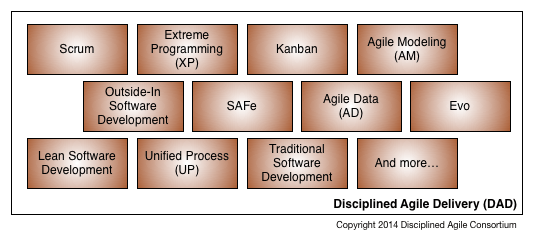
\includegraphics[scale=0.8]{hybrid1}
	\caption{DAD als hybrides Vorgehensmodell \cite{dadHybrid}}
	\label{fig:hybrid}
\end{figure}
\subsection{Phasen in DAD}
Allgemein kann gesagt werden das DAD aus drei Phasen besteht Inception, Construction und Transition (Abbildung \ref{fig:highlevellifecycle}). \smallskip
\begin{figure}[H]
	\centering
	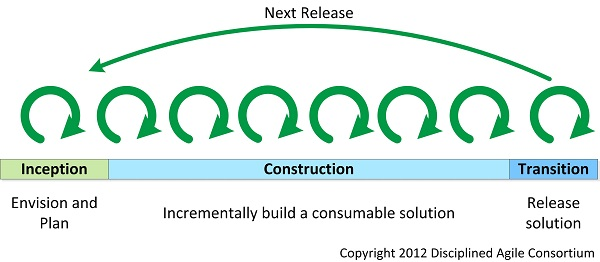
\includegraphics[width=\textwidth]{lifecycle}
	\caption{Highlevel Lifecycle von DAD\cite{lifecycleDAD}}
	\label{fig:highlevellifecycle}
\end{figure}\medskip
In der \textbf{Inception} Phase wird die Planung und Analyse des Projekts und dessen Ressourcen gemacht. Dies umfasst folgende Schritte:\smallskip
\begin{itemize}
	\item Initiales Team bilden
	\item Projekt Vision identifizieren
	\item Mit Stakeholder auf die Projekt Vision einigen
	\item Auf Unternehmensstrategie abstimmen
	\item Technische Strategie, initiale Anforderungen und initiale Release-Planung festlegen
	\item Arbeitsumfeld einrichten
	\item Finanzierung sichern
	\item Risiken identifizieren
\end{itemize}
\medskip
Die \textbf{Construction} Phase beinhaltet die eigentliche Entwicklung und das Testen, wo das entsprechende Vorgehensmodell eingesetzt wird.\smallskip
\begin{itemize}
	\item Eine verwendbare Lösung liefern
	\item Ändernde Bedürfnisse der Stakeholder adressieren 
	\item Näher an das einsetzbare Produkt herankommen
	\item Qualität verbessern oder höhere Qualität erarbeiten
	\item Architektur frühzeitig beweisen
	\item Arbeitsumfeld einrichten
\end{itemize}\medskip
Die \textbf{Transition} Phase betrifft Zieleinhaltung und Lieferung.
\begin{itemize}
	\item Einsatzfähigkeit der Lösung sicherstellen
	\item Empfangsbereitschaft der Stakeholder sicherstellen
	\item Lösung in produktive Umgebung liefern
\end{itemize}
\medskip

Auffallend ist hier das die Phasen identisch mit jenen von RUP (Rational Unified Process) sind\cite{rup}. DAD beinhaltet als nebst den Fundamenten von Scrum und XP auch jene von RUP.


\subsection{DAD als Scrum-basiertes Vorgehensmodell}

DAD als agiles Vorgehensmodell bedeutet eine erweiterte Scrum Vorgehensweise. Scrum wird dort erweitert wo es unzureichend definiert ist. In Abbildung \ref{fig:lifecycle} ist der komplette Lifecycle vom Scrum-basierten DAD dargestellt. Diese Abbildung scheint auf den ersten Blick sehr komplex. Bei genauerer Betrachtung ist aber ersichtlich, dass der Lifecycle viele Gemeinsamkeiten mit jenem von Scrum hat.


\begin{figure}[H]
	\centering
	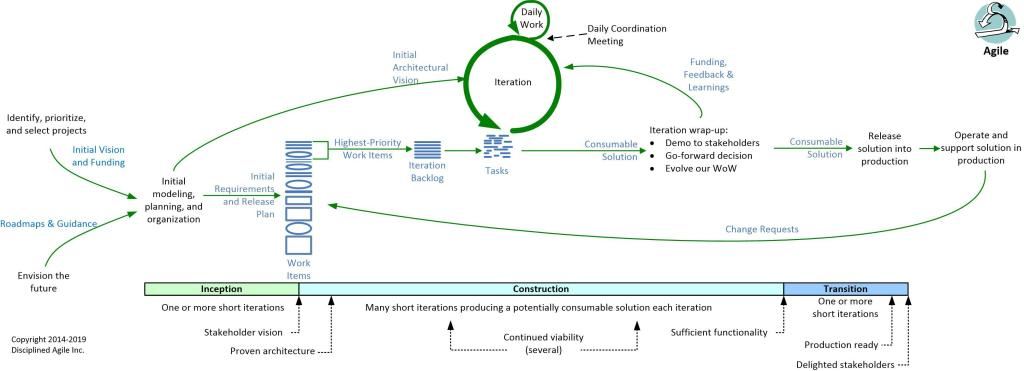
\includegraphics[width=\textwidth]{Lifecycle-DAD-Agile}
	\caption{Scrum-basiertes DAD Vorgehensmodells \cite{lifecycleDAD}}
	\label{fig:lifecycle}
\end{figure}\medskip

Dieses Vorgehensmodell bietet folgende interessante Aspekte:
\begin{itemize}
	\item Es ist iterationsbasiert.
	\item Es verwendet keine Scrum-Terminologie.
	\item Es zeigt Inputs ausserhalb des Vorgehensmodelles an.
	\item Es gibt eine Workitem-Liste, kein Product Backlog.
	\item Es enthält explizite Meilensteine.
\end{itemize}

\section{Anwendungsgebiete der beiden\newline Vorgehensmodelle}

Scrum wird häufig im Kontext von IT, Software-Entwicklung, Design oder Marketing, oder kontextähnlichen Gebieten eingesetzt. Jedoch ist wichtig, dass Scrum branchenunabhängig eingesetzt wird.

DAD wird im gleichen Kontext eingesetzt. Jedoch ist die Anwendung nur in komplexeren Unternehmenstrukturen sinnvoll. Zudem ist DAD geeignet als Mittel zur Transition von hierarchisch geprägten Strukturen zu agilen, selbstständigen Teams.
 
